\documentclass[tikz,border=12pt]{standalone}
\usepackage[T1]{fontenc}
\usepackage[scaled]{helvet}
\renewcommand{\familydefault}{\sfdefault}
\usetikzlibrary{positioning,arrows.meta,calc}

% ---------- Colors ----------
\definecolor{encC}{RGB}{110,110,110}     % encoder side
\definecolor{decC}{RGB}{52,101,164}      % decoder side
\definecolor{embC}{RGB}{206,92,0}        % encoder -> decoder link
\definecolor{noteC}{RGB}{60,60,60}

\tikzset{
	block/.style={draw, rounded corners=18pt, line width=1.2pt,
		minimum width=4.2cm, minimum height=2.6cm,
		font=\LARGE\bfseries},
	stagebox/.style={draw, rounded corners=5pt, line width=0.9pt, fill=white,
		minimum width=3.4cm, minimum height=0.75cm, font=\small},
	textbox/.style={draw, line width=1pt, minimum height=0.95cm,
		inner xsep=10pt, font=\large},
	flow/.style={-{Latex[length=3mm,width=2.6mm]}, line width=1.4pt},
	note/.style={align=center, text width=3.9cm, execute at begin node={\hyphenpenalty=10000},
		font=\footnotesize\bfseries, text=noteC},
	pointer/.style={-{Latex[length=2mm]}, thin, noteC},
}

\begin{document}
	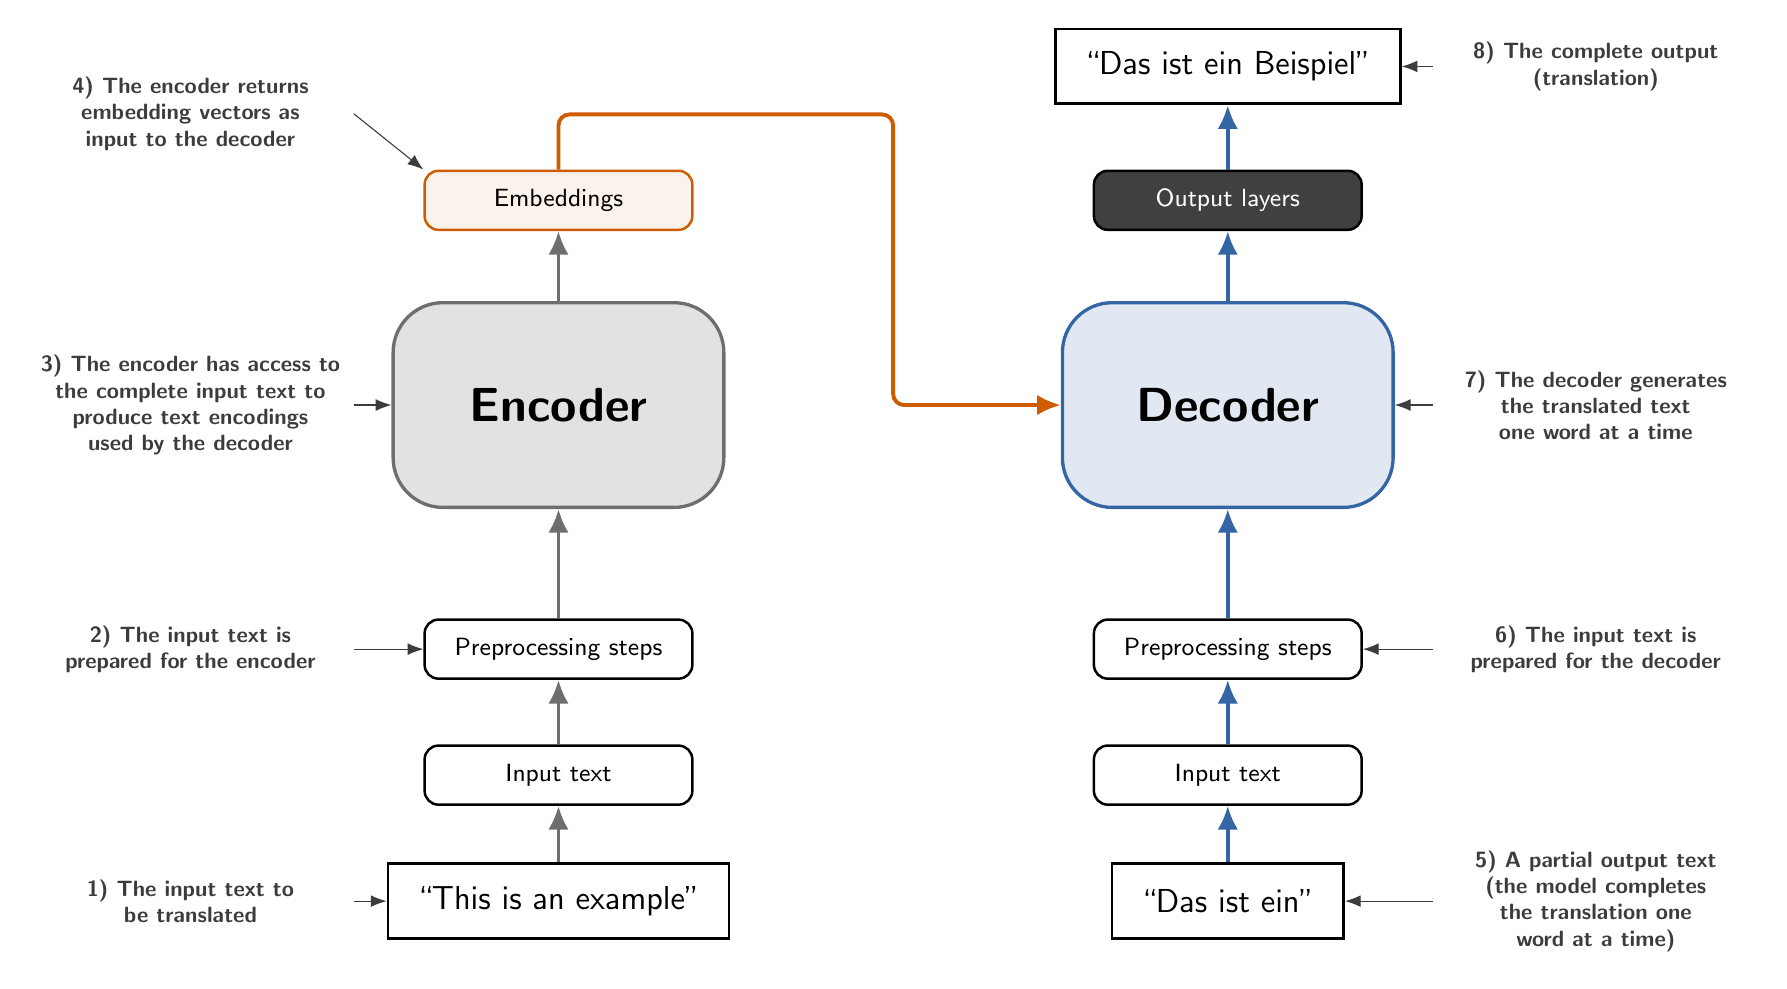
\begin{tikzpicture}
		
		% =============== ENCODER SIDE (x = 0) ===============
		\node[textbox] (qE)  at (0,-6.3) {``This is an example''};
		\node[stagebox]    (inE) at (0,-4.7) {Input text};
		\node[stagebox]    (prE) at (0,-3.1) {Preprocessing steps};
		\node[block, draw=encC, fill=encC!20] (enc) at (0,0) {Encoder};
		\node[stagebox, draw=embC, fill=embC!8] (emb) at (0,2.6) {Embeddings};
		
		\draw[flow, encC] (qE)  -- (inE);
		\draw[flow, encC] (inE) -- (prE);
		\draw[flow, encC] (prE) -- (enc);
		\draw[flow, encC] (enc) -- (emb);
		
		% =============== DECODER SIDE (x = 8.5) ===============
		\node[textbox] (qD)  at (8.5,-6.3) {``Das ist ein''};
		\node[stagebox]    (inD) at (8.5,-4.7) {Input text};
		\node[stagebox]    (prD) at (8.5,-3.1) {Preprocessing steps};
		\node[block, draw=decC, fill=decC!15] (dec) at (8.5,0) {Decoder};
		\node[stagebox, draw=black, fill=black!75, text=white] (out) at (8.5,2.6) {Output layers};
		\node[textbox] (final) at (8.5,4.3) {``Das ist ein Beispiel''};
		
		\draw[flow, decC] (qD)  -- (inD);
		\draw[flow, decC] (inD) -- (prD);
		\draw[flow, decC] (prD) -- (dec);
		\draw[flow, decC] (dec) -- (out);
		\draw[flow, decC] (out) -- (final);
		
		% =============== ENCODER -> DECODER LINK ===============
		\coordinate (mid) at ($(enc.east)!0.5!(dec.west)$);
		\draw[flow, embC, rounded corners=4pt]
		(emb.north) -- ++(0,0.7) -| (mid) -- (dec.west);
		
		% =============== ANNOTATIONS: encoder (left) ===============
		\node[note, anchor=east] (n1) at (-2.6,-6.3)
		{1) The input text to\\be translated};
		\draw[pointer] (n1.east) -- (qE.west);
		
		\node[note, anchor=east] (n2) at (-2.6,-3.1)
		{2) The input text is\\prepared for the encoder};
		\draw[pointer] (n2.east) -- (prE.west);
		
		\node[note, anchor=east] (n3) at (-2.6,0)
		{3) The encoder has access to the complete input text to produce text
			encodings used by the decoder};
		\draw[pointer] (n3.east) -- (enc.west);
		
		\node[note, anchor=east] (n4) at (-2.6,3.7)
		{4) The encoder returns embedding vectors as input to the decoder};
		\draw[pointer] (n4.east) -- (emb.north west);
		
		% =============== ANNOTATIONS: decoder (right) ===============
		\node[note, anchor=west] (n5) at (11.1,-6.3)
		{5) A partial output text (the model completes the translation
			one word at a time)};
		\draw[pointer] (n5.west) -- (qD.east);
		
		\node[note, anchor=west] (n6) at (11.1,-3.1)
		{6) The input text is\\prepared for the decoder};
		\draw[pointer] (n6.west) -- (prD.east);
		
		\node[note, anchor=west] (n7) at (11.1,0)
		{7) The decoder generates the translated text one word at a time};
		\draw[pointer] (n7.west) -- (dec.east);
		
		\node[note, anchor=west] (n8) at (11.1,4.3)
		{8) The complete output\\(translation)};
		\draw[pointer] (n8.west) -- (final.east);
		
	\end{tikzpicture}
\end{document}